\chapter{Introduction}

\section{Objective and Motivation}
The aim of this experiment is to investigate free, damped, and forced oscillations of a torsional pendulum. The focus is on determining the damping constant $\delta$ and the natural frequency $\omega_0$ using different methods. First, the period of undamped oscillations is measured, then the decay of the amplitude in damped oscillations is analyzed, and finally the resonance curves of forced oscillations are studied. Comparing the results from these different approaches allows an evaluation of the measurement methods and provides deeper insight into the dynamics of damped and driven oscillations.

\section{Theoretical Background}
A torsional pendulum can be modeled as a harmonic oscillator, which in practice is always subject to damping due to friction or other resistive forces. In this experiment, damping is introduced by an eddy current brake: electromagnets generate a magnetic field in which the moving pendulum induces eddy currents. According to Lenz’s law, these currents oppose the motion and decelerate the rotation of the pendulum.

\subsection{Free Harmonic Oscillator}
A free harmonic oscillator has no damping or external driving force. It is described by
\begin{equation}
\ddot{x} + \omega_0^2 x = 0,
\end{equation}
with the general solution
\begin{equation}
x(t) = a \cos(\omega_0 t + \varphi),
\end{equation}
where $a$ and $\varphi$ are constants determined by the initial conditions. The motion is purely sinusoidal with angular frequency $\omega_0$ and period
\begin{equation}
    T = \frac{2\pi}{\omega_0}.
    \label{eq:period_time}
\end{equation}
In this case, the energy of the system is conserved and oscillates between kinetic and potential energy without losses.

\subsection{Damped Oscillator}
Real oscillators are always damped due to resistive forces. Adding damping to the equation of motion yields
\begin{equation}
\ddot{x} + 2 \delta \dot{x} + \omega_0^2 x = 0.
\end{equation}
Here $\delta$ is the damping constant, which quantifies energy loss per cycle.  

Three regimes can be distinguished:
\begin{itemize}
    \item \textbf{Underdamped} ($\delta < \omega_0$): Oscillations occur with exponentially decaying amplitude. This is the relevant case for our experiment.
    \item \textbf{Critically damped} ($\delta = \omega_0$): The system returns to equilibrium without oscillating, and in the shortest possible time.
    \item \textbf{Overdamped} ($\delta > \omega_0$): The system also returns without oscillating, but more slowly than in the critical case.
\end{itemize}

For the underdamped case, the solution is
\begin{equation}
x(t) = e^{-\delta t} a \cos(\omega_f t + \varphi),
\end{equation}
where the damped angular frequency is
\begin{equation}
\omega_f = \sqrt{\omega_0^2 - \delta^2}.
\end{equation}
The amplitude decays exponentially according to
\begin{equation}
a(t) = a_0 e^{-\delta t}.
\end{equation}
The damping constant can be extracted from the half-life $t_{1/2}$ of the amplitude:
\begin{equation}
    \delta = \frac{\ln 2}{t_{1/2}}.
    \label{eq:damping_halftime}
\end{equation}

\subsection{Forced Oscillator}
When an external periodic driving torque acts on the system, the equation of motion becomes
\begin{equation}
\ddot{x} + 2\delta \dot{x} + \omega_0^2 x = A \omega_0^2 \cos(\omega t),
\end{equation}
with $A$ the driving amplitude and $\omega$ the driving angular frequency.  

The general solution consists of:
\begin{itemize}
    \item A \textbf{transient part}, proportional to $e^{-\delta t}$, which decays after a short time.
    \item A \textbf{steady-state part}, which oscillates with the driving frequency $\omega$ and dominates after the transient vanishes.
\end{itemize}

The steady-state solution is
\begin{equation}
x(t) = b(\omega) \cos(\omega t - \epsilon(\omega)),
\end{equation}
with amplitude
\begin{equation}
b(\omega) = \frac{A \omega_0^2}{\sqrt{(\omega_0^2 - \omega^2)^2 + (2 \delta \omega)^2}}.
\end{equation}

The maximum amplitude occurs at the resonance frequency
\begin{equation}
\omega' = \sqrt{\omega_0^2 - 2 \delta^2}.
\end{equation}
This value shifts below $\omega_0$ as damping increases.

\subsection{Resonance Curve}
The resonance curve $b(\omega)$ describes how the oscillation amplitude depends on the driving frequency. Key parameters:
\begin{itemize}
    \item \textbf{Resonance frequency:} $\omega'$, which decreases with stronger damping.
    \item \textbf{Resonance amplitude:} $b(\omega')$, which is smaller for stronger damping.
    \item \textbf{Half-width:} 
    \begin{equation}
        H = \omega_2 - \omega_1 \approx 2\delta,
        \label{eq:h_delta}
    \end{equation}
    a measure of frequency selectivity.
\end{itemize}

\begin{figure}[h!] 
    \centering 
    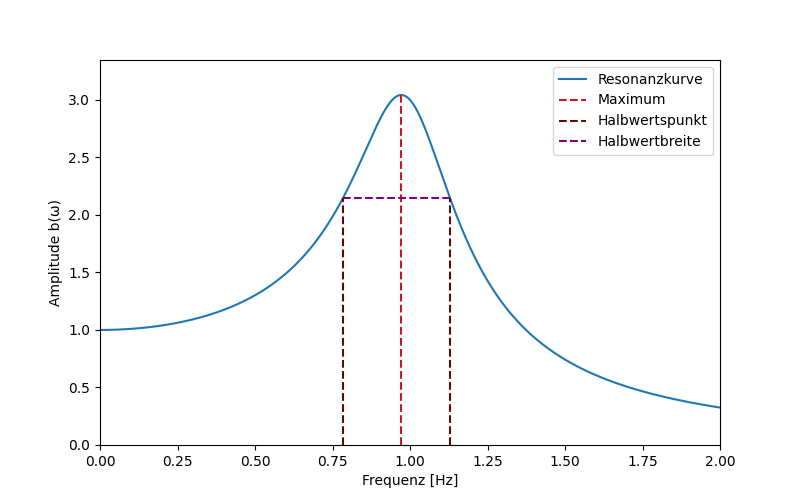
\includegraphics[width=0.5\textwidth]{img/13/Resonanzkurve_allgemein.png} 
    \caption{ Schematic resonance curve $b(\omega)$ of a damped, forced oscillator.} 
    \label{fig:resonancecurve} 
\end{figure}

The resonance amplification is
\begin{equation}
    \frac{b(\omega')}{b(\omega \to 0)} \approx \frac{\omega_0}{2 \delta}.
    \label{eq:reso_amp}
\end{equation}

\subsection{Quality Factor}
The sharpness of resonance is described by the quality factor
\begin{equation}
Q = \frac{\omega_0}{H} = \frac{\omega_0}{2 \delta}.
\end{equation}
Large $Q$ means weak damping, narrow resonance, and strong amplification. Small $Q$ means strong damping, broad resonance, and weak amplification.

\subsection{Forces Acting on the System}
The pendulum dynamics are governed by four torques:
\begin{itemize}
    \item \textbf{Restoring torque:} from torsional stiffness, proportional to angular displacement.
    \item \textbf{Damping torque:} from the eddy current brake, proportional to angular velocity.
    \item \textbf{Driving torque:} periodic torque applied by the motor in forced oscillation experiments.
    \item \textbf{Inertial torque:} due to the moment of inertia, opposing angular acceleration.
\end{itemize}

Their interplay determines whether the pendulum undergoes free, damped, or forced oscillation.

\begin{figure}[h!]
    \centering
    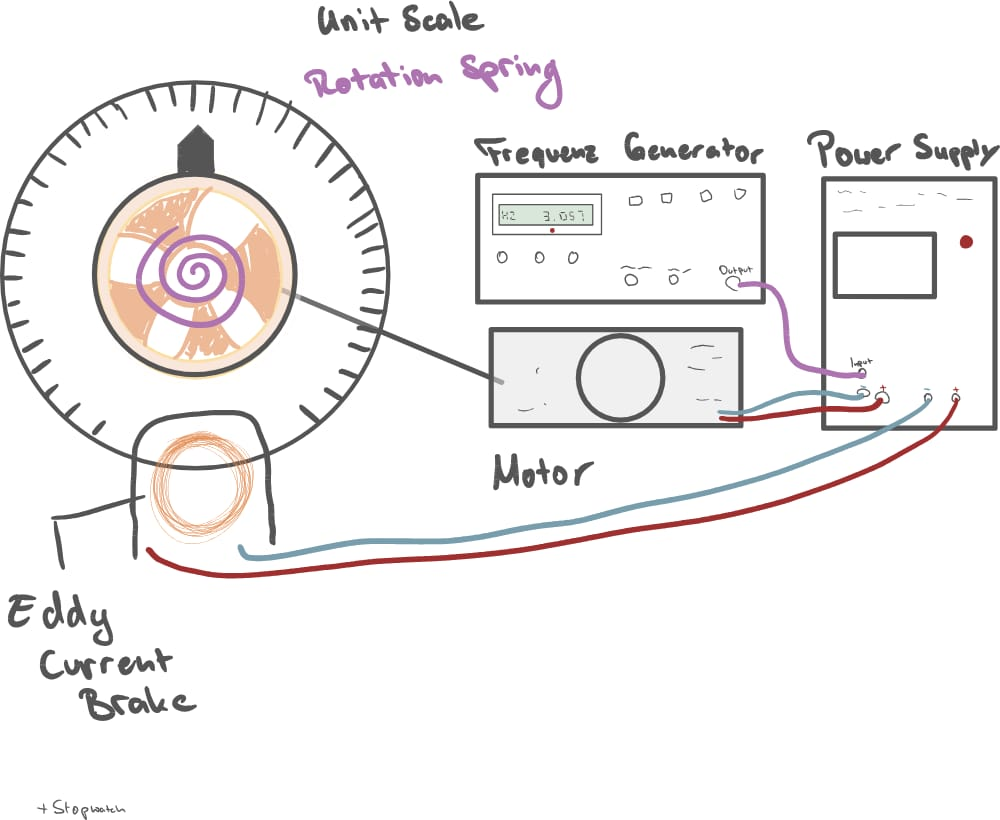
\includegraphics[width=0.75\textwidth]{img/13/aufbau.jpg}
    \onecolumn
    \caption{Schematic setup of the experiment}
    \twocolumn
\end{figure}